\title{Реализация общей\\
поддержки времени исполнения\\
для интерпретатора языка PostScript}
%
\titlerunning{Общая поддержка времени исполнения PostScript}
\author{Поздин Дмитрий Евгеньевич}
%
\authorrunning{Д.Е.Поздин} % abbreviated author list (for running head)
%
%%%% list of authors for the TOC (use if author list has to be modified)
\tocauthor{Д.Е.Поздин}
%
\institute{Санкт-Петербургский государственный университет\\
\email{podmev@gmail.com}}

\maketitle

\begin{abstract}
В данной работе решается задача построения и реализация общей среды исполнения для интерпретатора 
программ на языке PostScript с помощью языка Java. В неё входит стеки, локальная память, основные 
структуры языка (массивы, словари и строки) и механизм исполнения исходной программы. Эта задача 
рассматривается в контексте более общей~--- создания полноценного интерпретатора.
\end{abstract}

\section*{Введение}

PostScript~\cite{PLRM}~--- мощный, гибкий и платформонезависимый язык программирования, использующийся для вывода документов на печать. Основная идея языка состоит в построении модели текста и рисунков на чистой странице. Программы на PostScript могут обрабатывать как векторную, так и растровую графику. Разработан в 1982 году специалистами из Adobe Systems Джоном Уорноком и Чаком Гешке. Через некоторое время PostScript стал широко распространенным стандартом. Почти во всех современных компьютерных системах для печати документов присутствуют интерпретаторы PostScript, реализованые в виде аппаратных или программных компонентов. Основные реализации~--- Adobe PostScript\footnote{\url{http://www.adobe.com/products/postscript/}}, Ghostscript\footnote{\url{http://www.ghostscript.com/}}. Расширение файлов, соответствующее программам на языке PostScript~-- <<.ps>> или <<.eps>> (Encapsulated PostScript, вариант языка с некоторыми ограничениями).

PostScript~--- интерпретируемый, стековый язык со строгой динамической типизацией. В PostScript принят способ определения типов, при котором переменная связывается с типом в момент присваивания значения, а не в момент объявления. Таким образом, в различных участках программы одна и та же переменная может принимать значения разных типов. В PostScript принята обратная польская нотация, и при исполнении операций операнды берутся со стека. В PostScript отсутствуют зарезервированные слова, таким образом можно переопределить любую операцию. 

Для исполнения программ на языке PostScript необходим интерпретатор, который требуется реализовывать для каждого отдельного устройства. Это связано с различиями в машинной архитектуре. Для большинства машин есть реализация Java Virtual Machine~\cite{pjvms}. Если интерпретатор PostScript написан на Java, то исполнять программы на языке PostScript с его помощью можно на всех машинах, для которых реализована JVM.

В рамках курсовой работы решается задача построения и реализация общей среды исполнения для интерпретатора программ на языке PostScript с помощью языка Java. В неё входит стеки, локальная память, основные структуры языка (массивы, словари и строки) и механизм исполнения исходной программы. Эта задача рассматривается в контексте более общей~-- создание полноценного интерпретатора.  Для сравнения и анализа работы языка PostScript использовался интерпретатор Ghostscript.

%Задача исследовательской группы~--- написать интерпретатор языка PostScript на языке Java с использованием стандартных графических библиотек.

\section{Общая среда исполнения}
Далее будут представлены характерные особенности среды исполнения в соответствии со спецификацией языка PostScript\cite{PLRM}.

Общая среда исполнения манипулирует сущностями, которые в PostScript называются  объектами. Объекты хранят три поля: тип этого объекта, атрибуты (только для сложных объектов, исполняемый ли объект или литеральный и ограничение на чтение и запись) и значение объекта. Для сложных объектов (массивы, строки, словари, снимок локальной памяти) значение отделено от самого объекта и хранится в виртуальной памяти. При этом несколько сложных объектов могут разделять одно значение. Некоторые объекты трактуются как данные, такие как числа, булевы значения, строки, массивы. Другие объекты являются исполняемыми: имена, операторы и процедуры (исполняемые массивы). При этом строки, имена и массивы могут быть как данными, так и исполняемыми объектами.

Среда исполнения необходима для хранения промежуточного состояния в процессе исполнения исходной программы. Текущее состояние описывается четырьмя стеками и виртуальной памятью (там хранятся созданные объекты). Операторы могут использовать и изменять значения, хранящиеся в них.

\subsection{Стеки}
Интепретатор оперирует стеками операндов, словарей, графических состояний и исполнения. 
\begin{itemize}
\item Стек операндов содержит объекты, которые являются операндами и результатами действия операторов. 
\item Стек словарей содержит исключительно словари. Там всегда находится хотя бы три словаря: \texttt{systemdict, globaldict} и \texttt{userdict}. В словаре \texttt{systemdict} находятся все встроенные операторы с ключами, соответствующими их именам. Все словари, кроме \texttt{systemdict}, изменяемые, т.е. в них можно добавлять, изменять и удалять значения.
\item На стеке графических состояний находятся те состояния, котрые описывают параметры состояния графики, например, ширину линии, цвет, матрицу преобразования координат. Этот стек необходим для сохранения и восстановления состояния графики (операции \texttt{gsave, grestore}).
\item Интерпретатор использует стек исполнения для запоминания всех приостановленных процедур (контекстов исполнения). Процедуры в PostScript кладутся на стек исполнения. Когда интерпретатор достигает конца процедуры, она снимается со стека, и продолжается исполнение предыдущей процедуры с того места, где она  остановилась. Пока стек вызовов не пуст, исполняется очередной элемент процедуры, находящейся на вершине стека вызовов. По сути, процедура~-- это список объектов PostScript, которые надо исполнить.
\end{itemize}
 
\subsection{Виртуальная память}
В PostScript есть понятие глобальной и локальной виртуальной памяти. Поэтому при создании объекта можно выбрать, где его хранить~--- в локальной или глобальной памяти. Для простых объектов~--- значения хранятся сразу при объекте. Отличие локальной памяти от глобальной состоит в том, что состояние локальной памяти можно сохранять с помощью оператора \texttt{save} и восстанавливать с помощью оператора \texttt{restore}.


\subsection{Основные структуры языка PostScript}
Объекты в PostScript могут быть только следующих типов: \texttt{null, boolean, real, integer, name, mark, array, string, dictionary, file, save}. Также можно создавать только именованные объекты (объект лежит в словаре по некоторому имени) и, как частный случай, именованные процедуры, т.е. исполняемые массивы. В PostScript некоторые сложные структуры имеют свои особенности.

\subsubsection*{Массивы.}
Массивы хранят множество объектов, проиндексированное от \texttt{0} до \texttt{length-1}. При этом элементы массива могут быть любого типа. Добавлять элементы к массиву нельзя, т.е. он не динамический. Массивы в PostScript отличаются от массивов в других языках программирования тем, что подмассив некоторого массива хранит те же ссылки на объекты, что и оригинальный массив. Таким образом при изменении подмассива изменяется и сам массив. Исполняемый массив отличается от литерального.  Литеральный массив трактуется просто как набор данных, в то время как исполняемый массив (или по-другому процедура) это набор объектов, которые необходимо исполнить при вызове этой процедуры.

\subsubsection*{Строки.}
Строка хранится посимвольно, при этом каждый символ описывается числом от 0 до 255. Строки и массивы похожи: изменение подстроки изменяет оригинальную строку. Также есть и отличие: при операции \texttt{restore} значения строк не восстанавливается.

\subsubsection*{Словари.}
Словарь~--- это такая структура, в которой по некоторому уникальному ключу хранится значение. При этом и значение, и ключ являются объектами, т.е. могут быть числом, строкой, массивом, именем и т.д. Единственное чем не может быть ключ, это меткой (открытие, закрытие массива), \texttt{null} (т.е. пустой объект) и оператором.

\subsubsection*{Метки.}
В языке PostScript есть несколько разных типов меток для обозначения начала или конца некоторой структуры. <<$$<<$$>>, <<$$>>$$>>~--- метки для обозначения, соответственно, начала и конца записи словаря. <<\texttt{[}>>, <<\texttt{]}>> используются для массива. <<\texttt{\textbraceleft}>>, <<\texttt{\textbraceright}>> используются для исполняемого массива.
\subsection{Сборка мусора}
В языке PostScript поддерживается сборка мусора, как в глобальной, так и в локальной памяти. В локальной памяти сборка мусора производится для всех объектов, созданных после последней операции \texttt{save}.

\section{Реализация общей поддержки времени исполнения}
Общая поддержка времени исполнения была выполнена в соответствии с требованиями, указанными в спецификации.

\subsection{Объекты}
Объекты в интерпретаторе представляются классом \texttt{PSObject} с тремя полями: тип, атрибуты, значение. Значение объекта описывается классом \texttt{Value}.

Отличительной особенностью языка является операции \texttt{save} и \texttt{restore}. Они позволяют сохранять и восстанавливать состояние локальной памяти. Именно поэтому было решено сделать значения всех объектов в интерпретаторе неизменяемыми для того, чтобы сохраненные значения не перезаписывались. Например, при изменении элемента массива по индексу создается новый массив с заменённым значением по индексу.

\subsection{Общая среда исполнения}
Для реализации общей среды исполнения был создан основной класс \texttt{Runtime}. Он содержит стеки и локальную память в качестве полей. Каждый из них реализован отдельным классом. Также есть три поля, соответствующие трем стандартным словарям (\texttt{systemdict, globaldict} и \texttt{userdict}), несмотря на то, что к ним есть доступ через стек словарей. Поля были созданы для быстрого доступа к этим словарям. Есть ещё поле \texttt{isGlobal}~-- булевый флаг, описывающий, в какую память записываются объекты: в локальную или глобальную.

Для стеков в классе \texttt{Runtime} создан набор публичных методов для работы с ними. Например, \texttt{pushToOperandStack(), popFromOperandStack(), peakFromOperandStack(), getOperandStackSize()}. 


\subsection{Виртуальная память}
Для сложных объектов была создана двухуровневая адресация в локальной памяти, чтобы сложные объекты могли разделять одни значения. В объекте хранится не само значение, а только ссылка~-- \textit{локальная} или \textit{глобальная}. В локальной ссылке хранится номер из локальной виртуальной памяти. И уже по номеру в локальной памяти хранится необходимое значение. В глобальной же ссылке хранится сразу значение сложного объекта.

\subsubsection*{Локальная виртуальная память.}
Локальная память представляется классом \texttt{LocalVM}. В нем хранится таблица значений сложных объектов (map \texttt{HashMap<Integer, CompositeValue>}). Также есть поле \texttt{maxInt}, характеризующее индекс, по которому можно записать следующее сложное значение. Основные методы класса~--- \texttt{add()}, \texttt{remove()} и \texttt{setNewValueAtIndex()}, соответственно добавляющий значение метод, удаляющий и изменяющий значение по индексу. Также реализовано глубокое клонирование, в котором создается новая таблица по значениям старой. Сами значения не клонируются. Клонирование необходимо для создания снимка локальной памяти во время операции \texttt{save}. 

\begin{lstlisting}[label=LocalVM,caption=Интерфейс класса LocalVM, frame = none, language = Java]
public class LocalVM {
    private Map<Integer,CompositeValue> map=new HashMap<Integer,CompositeValue>();
    private Set<Integer> initSet = new HashSet<Integer>();
    private Set<Integer> stringSet = new HashSet<Integer>();
    private int maxInt = 0;
    public int add(CompositeValue value) {...}
    public void remove(int index) {...}
    public void setNewValueAtIndex(int index, CompositeValue value) {...}
    public boolean contains(Value value) {...}
    public CompositeValue get(int index) {...}
    public void clear() {...}
    public void initDefaultKeys() {...}
    public void clearGarbage(Set<Integer> rootSet) {...}
    public void updateStringValues(LocalVM newLocalVM) {...}
    public LocalVM clone() {...}
    ...
}
\end{lstlisting}

\subsection{Сборка мусора}
При использовании виртуальной памяти и создании в ней новых значений возникает огромное количество <<мусора>>~-- объекты, которые никогда больше не будут использоваться. Поэтому в интерпретаторе необходимо регулярно во время исполнения производить сборку мусора.

Сборка мусора в глобальной памяти осуществляется сборщиком мусора Java. Поэтому интересен случай только локальной памяти, когда сборщик мусора Java не может удалять мусор, т.к. значения хранятся в таблице в локальной памяти, и на них всегда есть ссылка.

В интерпретаторе реализована консервативная сборка мусора. Корневое множество определяется в методе \texttt{getRootSet()} в классе \texttt{Runtime}. Для этого обходятся три стека операндов, словарей и исполнения. Если значения объекта хранится в локальной памяти, то индекс, по которому он хранится, добавляется в корневое множество. Если при этом объект~--- массив или словарь, то проверяется рекурсивно, лежат ли все компоненты этих структур в локальной памяти.

Сборка мусора запускается через определенное количество исполнений объектов (сейчас это число равно 10000) и  перед сохранением (для того, чтобы не хранить в снимке значения в локальной памяти, которые являются мусором).  При сборке мусора приостанавливается исполнение процедур. Сборка состоит из двух шагов: определение корневого множества и, собственно, удаление мусора в локальной памяти (вызов метода \texttt{cleanGarbage()} из класса \texttt{LocalVM}).

В качестве параметра в метод \texttt{cleanGarbage()} передается корневое множество~--- это множество индексов локальной памяти, которые ссылаются на значения, использующиеся на данный момент в программе. Этот метод удаляет все записи, которые не находятся в корневом множестве и <<\textit{стартовом множестве}>> (\texttt{initSet}). Стартовое множество~--- это все объекты, созданные до последней операции \texttt{save}, их не следует удалять по спецификации языка. 

Таким образом, после сборки мусора в локальной памяти остаются только те значения объектов, к которым есть доступ через стеки, или которые были созданы до последней операции сохранения.

\subsection{Процедуры}
Процедура  описывает контекст исполнения. Все процедуры унаследованы  от  класса \texttt{Procedure} (рис.~\ref{procedures}). По сути, процедура~--- это список объектов PostScript, которые надо исполнить. У процедур есть два основных метода \texttt{hasNext()} и \texttt{execNext()}. Первый соответственно выдает булево значение, есть ли следующий объект для исполнения, а второй исполняет очередной объект. Для каждой процедуры по-своему определяются два метода \texttt{hasNext()} и \texttt{next()}. Последний возвращает очередной объект процедуры. Все особенности исполнения отдельных объектов разных типов описаны в методе \texttt{execObject(PSObject)}.

\begin{lstlisting}[label=Procedure-listing,caption=Абстракный класс Procedure, frame = none, language = Java]
public abstract class Procedure {
    private int procDepth = 0;
    ...
    public abstract boolean hasNext();
    protected abstract PSObject next(); 
    private void execObject(PSObject psObject) {...}
    public void execNext() {...}
    ...
}
\end{lstlisting}

\subsubsection*{Иерархия процедур.}

\begin{figure}[t]
\center{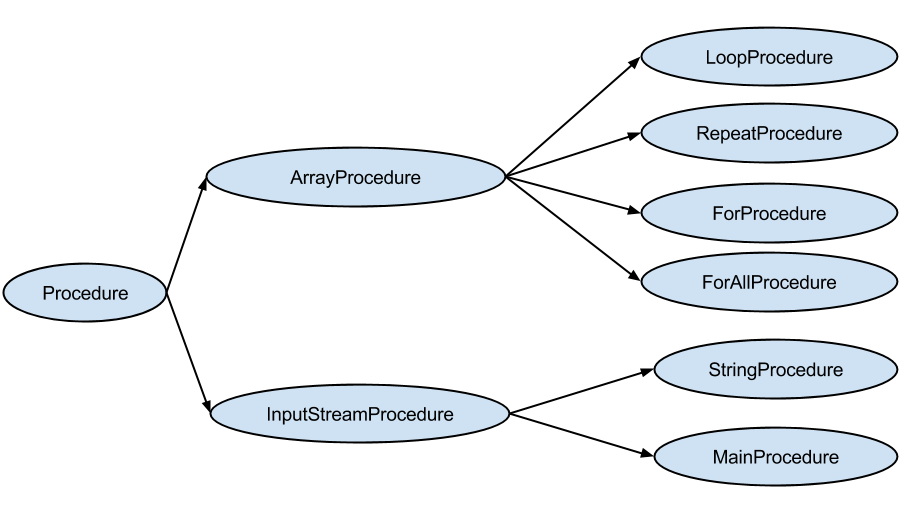
\includegraphics[width=\linewidth]{Pozdin/ProcedureTree.png}}
\caption{Иерархия процедур}\label{procedures}
\end{figure}

При создании всем процедурам дается имя. Процедуры делятся на два типа: в основе одних лежит массив объектов (\texttt{ArrayProcedure}), в основе других~-- текст программы \texttt{InputStreamProcedure}. От последней наследуются две процедуры: \texttt{MainProcedure} и \texttt{StringProcedure}. \texttt{MainProcedure}~--- главная процедура, которой передается файл с программой на языке PostScript. Он обрабатывается сканером \texttt{Yylex}, сгенерированным при помощи генератора лексических анализаторов JFlex\footnote{\url{jflex.de}}. Для \texttt{MainProcedure} очередной объект конструируется из токена, полученного сканером, и возвращается в методе \texttt{next()}. Сам токен характеризуется типом и строкой, содержащей текст токена. Поэтому для каждого типа токена получаются разные объекты. Аналогично работает процедура \texttt{StringProcedure}. Она необходима для исполнения внутри программы строк, которые являются подпрограммами на языке PostScript.

От класса \texttt{ArrayProcedure} наследуются \texttt{LoopProcedure, ForProcedure, RepeatProcedure} и \texttt{ForAllProcedure} для соответствующих операторов. \texttt{LoopProcedure} перебирает все элементы массива, а после начинает сначала, до тех пор пока не прервется оператором \texttt{exit}. По сути, это аналог \texttt{while(true)} и \texttt{break} в других языках программирования. Процедура \texttt{ForProcedure} на каждой итерации выдает значение переменной, которое инкрементируется, а после все элементы массива. Это выполняется до тех пор пока выполнено неравенство~-- условие на переменную. Для \texttt{ForAllProcedure} в начале  итерации выдается очередной элемент из дополнительной структуры, которая ей передается, а уже после все элементы из массива, что похоже на \texttt{foreach} в высокоуровневых языках. В качестве итерируемой структуры может выступать массив, словарь (в~этом случае итерация идет по всем ключам и значения) или строка (выступает, как массив символов). В случае \texttt{RepeatProcedure} итераций по массиву ровно столько, сколько передается в оператор \texttt{repeat}, т.е. какое-то натуральное число раз.

\subsubsection*{Исполнение процедур.}
Основным методом управления исполнения программы является метод \texttt{executeCallStack()} (см. листинг~\ref{ExecCallStack-listing}). В нем происходит выполнение очередного объекта процедуры, находящейся на вершине стека исполнения.  В начале работы на пустой стек исполнения кладётся одна процедура \texttt{MainProcedure} с файлом исходной программы. В процессе исполнения на стек исполнения кладутся дополнительные процедуры. Работа завершается при опустошении стека исполнения.

\begin{lstlisting}[label=ExecCallStack-listing,caption=Механизм исполнения, frame = none, language = Java]
    public void executeCallStack() {
        while (!callStack.isEmpty()) {
            Procedure topProcedure = callStack.peek();
            if (topProcedure.hasNext()) {
                executionCount++;
                topProcedure.execNext();
                if (executionCount % executionsBeforeGarbageCleaning == 0) {
                    localVM.clearGarbage(getRootSet());
                }
            } else {
                topProcedure.procTerminate();
                popFromCallStack();
            }
        }
    }
\end{lstlisting}


\subsection{Основные структуры данных}
При реализации основных структур, таких как массивы, строки и словари, нельзя было использовать стандартные структуры из языка Java. Например, для массива логично было бы использовать \texttt{PSObject[]}, т.е. стандартный массив, или \texttt{ArrayList<PSObject>}. Для строк~-- стандартный \texttt{String}, а для словарей~-- \texttt{HashMap<PSObject,PSObject>}. При таких реализациях структур PostScript не выполнялись бы некоторые условия, описанные в обзорной части, и свойство неизменяемости для сложных значений.

\subsubsection*{Массивы.}
Значение массива представляется классом \texttt{PSArray}. Для того, чтобы массивы могли разделять значения, и при изменении одного изменялся, соответственно, другой массив, был создан дополнительный класс \texttt{ArrayElement}. Этот класс имеет единственное поле \texttt{PSObject}. Есть также методы для получения этого объекта и изменения. \texttt{ArrayElement}~--- <<обертка>> для хранения объектов в массиве. В классе \texttt{PSArray} хранится в качестве поля \texttt{ArrayElement[]}. 

Если два массива имеют общие значения, то это значит, что в этих массивах хранится некоторое количество одних и тех же объектов класса \texttt{ArrayElement}. Это возможно, например, при взятии подмассива (операция \texttt{getInterval}). При изменении массива изменяется содержимое конкретных \texttt{ArrayElement}.

\subsubsection*{Строки.}
Аналогично с массивами работают строки (\texttt{PSString}). Для хранения каждого символа используется один байт, хранящийся в виде поля в классе \texttt{StringElement}. Это необходимо для того, чтобы строки могли разделять значения.

\subsubsection*{Словари.}
За основу словаря было взято обычное AVL-дерево~\cite{cormen} с балансировкой, в каждом узле которого хранится ключ, значение и две ссылки на левое и правое поддерево. Особенности реализации состоят в том, что дерево неизменяемое, т.е. операции добавление, удаление и изменения элемента возвращают новое дерево. Вместо того, чтобы полностью создавать измененное дерево, мы переиспользуем те поддеревья старого дерева, которые не нужно менять. Итого, при операции мы создаем  ровно столько новых вершин в дереве, сколько содержится в пути от корня до вершины, с которой происходит действие, и еще полностью создается поддерево с этой вершиной в качестве корня.

Для того чтобы искать, добавлять и балансировать в дереве необходимо уметь сравнивать ключи (напомним, что ключами может быть практически любой \texttt{PSObject}). <<Естественное>> сравнение есть только у чисел и имен (в имени содержится строка). Необходимо было создать <<искусственное>> сравнение для всех объектов. Поэтому при сравнении сначала сравниваются типы объектов (все типы упорядочены), а после, если объекты разного типа, то используется сравнение внутри типа. Для сравнении объектов, чьи значения находится в локальной памяти, просто сравниваются индексы, по которому они хранятся. Для глобальной памяти сделан искусственный индекс, по которому мы и идёт сравнение. Отметим, что при использовании в качестве ключей объектов, в которых хранятся строки (\texttt{PSString}), они автоматически конвертируются в имена (\texttt{PSName}) в соответствии со спецификацией.

\subsection{Механизм исполнения объектов}
Исполнение объектов в интерпретаторе реализовано в методе  \texttt{execObject(PSObject)} класса \texttt{Procedure}. Объект исполняется по-разному в зависимости от его типа, атрибутов и вложенности процедур. Исполнение всех объектов, кроме имен, строк, массивов, меток и операторов, осуществляется путем помещения этого объекта на стек операндов. Когда объект литеральный, это означает, что он трактуется как часть данных и при выполнении кладётся на стек. Если вложенность процедур ненулевая, то объект в любом случае кладется на стек, в этом случае он рассматривается как литеральный объект. Рассмотрим оставшиеся типы объектов, когда нет вложенности процедур.
\begin{itemize}
\item  Для метки начала словаря, массива или процедуры на стек кладется просто сама метка.
Если при исполнении процедуры встретилась метка начала процедуры (в языке PostScript для этого используется фигурная скобка), то глубина вложенности увеличивается, при встрече метки <<\}>>~--- глубина уменьшается. Когда встречается метка конца структуры, то вызывается соответствующий оператор, который компонует набор объектов на стеке в сложный объект.

\item Исполняемый массив выполняется добавлением на стек исполнения новой процедуры (\texttt{ArrayProcedure}), инициализированной этим массивом. Таким образом, следующий исполняемый объект~--- первый объект из этого массива, поскольку новая процедура лежит на вершине стека исполнения. Литеральный же массив, как уже упоминалось, кладется на стек операндов.

\item Исполняемая строка выполняется добавлением на стек исполнения новой процедуры (\texttt{StringProcedure}), инициализированной этой строкой. Это есть не что иное, как исполнение подпрограммы.

\item При исполнении оператора выполняется тот код, описанный в этом операторе. Эти действия могут  влиять на отображения графики и состояния стеков, виртуальной памяти.

\item Имена, наиболее мощное средство языка, исполняются следующим образом. В случае литерального имени оно просто кладется на стек операндов. Для исполняемого имени необходимо найти соответствующие ему значение и его исполнить. Поиск происходит по словарям из стека словарей сверху вниз. Если объект найден, то он тут же исполняется в соответствии с типом. Напомним, что системный словарь (\texttt{systemdic}) находится в самом низу стека словарей. Поэтому, если для  оператора перезаписано действие по его имени в каком-нибудь словаре на стеке словарей, то будет исполняться перезаписанное действие (это может быть любой объект, в том числе и исполняемый массив).
\end{itemize}


\subsection{Операторы}
Встроенные операторы являются неотъемлемой частью общей среды исполнения. Именно с помощью них при исполнении программы происходит взаимодействие с составляющими среды исполнения. Оператор реализован, как один из типов объектов. Все конкретные реализации операторов унаследованы от класса \texttt{Operator} (см. листинг \ref{Operator-listing}).

\begin{lstlisting}[label=Operator-listing,caption=Абстракный класс Operator, frame = none, language = Java]
public abstract class Operator extends SimpleValue {
    ...
    public abstract void execute();
    public abstract PSName getDefaultKeyName();
    ...
} 
\end{lstlisting}
Для каждого оператора действие, которое необходимо выполнить, реализовано в методе \texttt{execute()}. Предопределенное имя оператора возвращается в методе \texttt{getDefaultKeyName()}.

В языке PostScript предусмотрено огромное количество операторов. В некоторых существующих интерпретаторах реализованы далеко не все из них. Чтобы легче было работать с операторами, они были разбиты на несколько тематических групп. Вот некоторые из них: арифметика, логические операторы и сравнения, операторы для работы с атрибутами, разными сложными объектами, стеками, виртуальной памятью, графические операторы, операторы потока управления.

Некоторые операторы довольно примитивны, например, для арифметики и логики взяты просто соответствующие операторы языка Java и библиотеки \texttt{math}. 

\iffalse Поэтому остановимся на тех операторах, которые заслуживают внимания.
\subsubsection*{Операторы для работы со словарями.}
\begin{itemize}
\item Наиболее важный оператор из этой группы~--- \texttt{def}. Он служит для он служит для инициализации переменных и процедур.

\texttt{/a [1 2 3] def \% Инициализация массивом переменной a \\
/b \{2 3 add\} def \% Создание процедуры b, складывающей 2 и 3
}

При вызове \texttt{def} берется со стека 2 объекта: первый будет ключом, второй~--- значением. Эта пара кладется в словарь, находящегося на вершине стека словарей.
\end{itemize}

\subsubsection*{Операторы потока управления.}
\begin{itemize}
\item \texttt{forall}
\item \texttt{for}
\item \texttt{repeat}
\item \texttt{loop}
\end{itemize}
\fi
\section{Результаты}
Результатом курсовой работы является часть интерпретатора, которая отвечает за поддержку времени исполнения. Интерпретатор позволяет исполнять программы на языке PostScript, результат выводится в отдельном окне в виде картинки. Для определения корректности исполнения работы интерпретатора происходило тестирование на наборе тестов. Рассмотрим несколько примеров тестов.

\begin{figure}[t]
\center{
\includegraphics[width=0.5\linewidth]{Pozdin/rectangles.png}}
\caption{Результат интерпретации программы}\label{rectangles}
\end{figure}

\subsection{Пример 1. Квадраты}
В этом примере (см. листинг~\ref{rectagles_ps} и рис.~\ref{rectangles}) используется исполняемый массив, записанный в словарь по имени <<\texttt{box}>> (\texttt{\textbackslash box \{...\} def}). Эта процедура, которая создает квадрат с определенной позиции (её необходимо задать перед процедурой). Квадрат строится с помощью ломаной из трёх отрезков и её замыкания. Далее в программе трижды исполняется следующее: устанавливается текущая позиция, исполняется процедура \texttt{box}, изменяется цвет цвет раскраски на градацию серого и происходит сама заливка. В конце исполняется оператор \texttt{showpage} для отображения результата.
\begin{lstlisting}[label=rectagles_ps,caption=Три квадрата, frame = none, language = PostScript]
/box { 72 0 rlineto 0 72 rlineto -72 0 rlineto closepath} def
252 324 moveto box 0 setgray fill
270 360 moveto box 0.4 setgray fill
288 396 moveto box .8 setgray fill
showpage 
\end{lstlisting}

\begin{figure}[t]
\center{
\includegraphics[width=0.5\linewidth]{Pozdin/mandelbrotset.png}}
\caption{Результат интерпретации программы}\label{mandelprotset}
\end{figure}

\subsection{Пример 2. Множество Мандельброта}
Рассмотрим более сложный пример (см. листинг~\ref{mandel_ps} и рис.~\ref{mandelprotset}) --- построение множество Мандельброта. Для этого определяются процедуры действий с комплексными числами (здесь это массив из двух чисел). В основной части программы используются циклы, условные операторы, прерывания циклов. При этом создается огромное количество процедур из-за тройной вложенности циклов.

Этот тест не выполнялся без использования сборки мусора, поскольку память переполнялась, в результате картинка не могла дорисоваться. Время исполнения  довольно значительное -- 44 секунды. В то время как интерпретатор GhostScript тратит на этот тест 3 секунды.

\begin{lstlisting}[label=mandel_ps,caption=Множество Мандельброта, frame = none, language = PostScript]
100 500 translate
/origstate save def
/maxiter 15 def
/ld {load def} bind def
/m /moveto ld /g /setgray ld
/dot { currentpoint 1 0 360 arc fill } bind def
% complex manipulation
/complex { 2 array astore } def
/real { 0 get } def
/imag { 1 get } def
/cmul { /a exch def /b exch def
    a real b real mul
    a imag b imag mul sub
    a real b imag mul
    a imag b real mul add
    2 array astore
} def
/cadd { aload pop 3 -1 roll aload pop
    3 -1 roll add
    3 1 roll add exch 2 array astore
} def
/cconj { aload pop neg 2 array astore } def
/cabs2 { dup cconj cmul 0 get} def
% mandel
200 100 translate
-200 1 100 { /x exch def
  -100 1 100 { /y exch def
    /z0 0.0 0.0 complex def
    0 1 maxiter { /iter exch def
    x 100 div y 100 div complex
    z0 z0 cmul
    cadd dup /z0 exch def
    cabs2 4 gt {exit} if
    } for
    iter maxiter div g
    x y m dot
  } for
} for
showpage
origstate restore
\end{lstlisting}

\subsection{Достоинства}
К достоинствам можно отнести создание всех компонентов среды исполнения, для которой корректно работают все операторы. Особо стоит отметить реализацию исполнения процедур, для каждой из которых в каждый момент исполнения известно только, какой следующий объект необходимо исполнить. Реализовано большинство операторов  --- более 130.

\subsection{Недостатки}
Главный недостаток -- время работы. Это заметно только на объемных тестах, где используется огромное количество объектов и процедур. Следующий недостаток, реализация массива. В ней есть дополнительная абстракция, которая может быть лишняя (\texttt{ArrayElement}), из-за неё теряется свойство неизменяемости, но становится возможным для массивов иметь одинаковые элементы. На данный момент, теряются связи между массивами после восстановления состояния локальной памяти. Не реализована поддержка использования файлов как объектов и операторов для работы с ними. Также никак не поддерживается обработка ошибок и исключений.

\section*{Заключение}
\addcontentsline{toc}{section}{Заключение}

В рамках курсовой работы разработана общая поддержка времени исполнения для интерпретатора программ на языке PostScript.
В среду исполнения входят:
\begin{itemize}
\item стеки операндов, словарей, графических состояний и исполнения;
\item локальная память с двухуровневой адресацией;
\item сборка мусора в локальной памяти консервативным способом;
\item механизм исполнения объектов языка;
\item процедуры (находятся на стеке исполнения);
\item основные структуры (массивы, строки, словари);
\item системные словари и встроенные операторы.
\end{itemize}

Разработанный интерпретатор работает на входных тестах, и в нем реализовано все компоненты среды исполнения, как того требует спецификация. Была произведена работа по поддержке большинства операторов.

\begin{thebibliography}{99}

\bibitem{PLRM}
Спецификация языка Postscript. PostScript Language reference. \\
Adobe Systems. 1999\\
\url{http://www.adobe.com/products/postscript/pdfs/PLRM.pdf}

\bibitem{pjvms}
Tim Lindholm, Frank Yellin, Gilad Bracha, Alex Buckley.
The Java Virtual Machine Specification.
Java SE 7 Edition, 2013. \\
\url{docs.oracle.com/javase/specs/jvms/se7/jvms7.pdf}

\bibitem{cormen}
 Томас Х. Кормен, Чарльз И. Лейзерсон, Рональд Л. Ривест, Клиффорд Штайн.
Алгоритмы: построение и анализ.
Второе издание, 2006

\end{thebibliography}
